\subsection{Zielplatform}
    Die neu zu implementierende Kontaktsuche zu soll im Relaunch der unternehmensinternen Administration umgesetzt werden.

    \subsubsection{Architektur}
        Diese folgt einem modularen Ansatz und stellt Webanwendungen nach dem MVC-Prinzip bereit. Dabei wird die Software in 3 logische Komponenten unterteilt: Die View (Ansicht, welche beispielsweise im Browser angezeigt wird), das Model (übernimmt backendseitige Programmlogik wie Datenbankabfragen oder Be- und Verrechnung von Daten) und den Controller (dient als Schnittstelle zwischen Model und View und reicht Anfragen und Antworten zu der jeweiligen Gegenseite durch).

        \vspace{0.5cm}
        \begin{figure}[h]
            \centering
            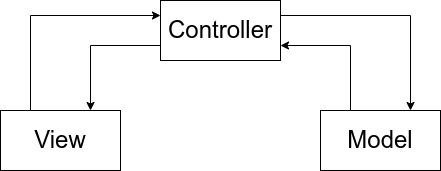
\includegraphics[width=0.5\textwidth]{MVC.jpg}
            \caption{Model View Controller - schematische Darstellung}
        \end{figure}

    \subsubsection{Technologien}
        Die zugrundeliegenden Technologien sind einerseits PHP in der Verion 8.0 mit dem Framework \glqq Laravel\grqq{} in Version 8.72.1, einer MySQL Datenbank in Version 5.5.62 und Node.JS zum Bereitstellen des Frontends. Die auszuliefernden Dateien liegen als Typescript-Quelldateien vor. Clientseitig kommt das Javascript-Framework \glqq React\grqq{} und die CSS-Bibliothek \glqq Bootstrap\grqq{} zum Einsatz.\\
        Die Entscheidung, PHP und Laravel zu verwenden, viel mit Hinblick auf den Relaunch der Unternehmensportale \glqq Print24\grqq{} und \glqq Easyprint\grqq{}, da dadurch eine unternehmensweite einheitliche Basis in den zugrundeliegenden Technologien besteht. Das gleiche gilt für die Wahl des Datenbankmodells, was noch näher in Abschnitt 4.1.3 erläutert wird. Die Wahl für Typescript anstelle von Javascript viel ebenfalls in der Planungsphase des Admin-Relaunches. Durch den objektorientierten Ansatz und die vorhandene Typensicherheit weißt ist der resultierende Code robuster und sicherer als reiner Javascript-Code. Als Quasi-Ersatz für das im Altsystem genutzte Template Toolkit kommt Node.JS zum Einsatz. Dies rendert die Websites der Anwendung mit dynamischen Inhalten bereits serverseitig vor und liefert sie dem Client in fertiger Form aus.\\
        Auf Clientseite wird React verwendet, welches durch das Einbinden von zusätzlichen Modulen schnell, einfach und zielgerichtet in dessen Funktionalität angepasst und erweitert werden kann. die Module sind hierbei nicht global verfügbar, sondern müssen explizit in jeder App eingebunden werden. Dies gewährleistet eine erhöhte Sicherheit der Gesamtumgebung, da eventuelle Schwachstellen in Modulen nur dann eine Gefahr darstellen, wenn diese auch aktiv in einer Anwendung genutzt wird. Weiter reduziert sich durch React der zu schreibende Code auf ein Minimum, was der Wartbarkeit der Anwendung durchaus zugute kommt. Außerdem können dadurch auch dynamische Inhalte besser verarbeitet und dargestellt werden.\\
        Für das Styling der Seite fiel die Wahl auf das von Twitter entwickelte freie CSS-Framework Bootstrap. Dieses ist global verfügbar imd bringt eine einfach zu lernende Syntax zum Einbinden CSS-Klassen und eine vielseitige Auswahl bereits vordefinierter Styling-Klassen mit sich. Durch die einheitliche Verwendung von Bootstrap wird sichergestellt, dass im gesamten Admin-Relaunch ein einheitlicher optischer Stil vorherrscht. Gleichzeitig kommt dies wieder der Wartbarkeit und einer reduzierten Codebasis zugute, da dadurch das manuelle Anlegen und Pflegen von CSS-Quelldateien und -Klassen entfällt.

    \subsubsection{Datenbankmodell}
        Die Mitarbeiterdaten werden bereits in einer relationalen MySQL Datenbank gespeichert und gepflegt. Die Wahl für dieses Datenbankmodell ist darin begründet, dass durch dieses Design Redundanzen in dem Datensätzen vermieden werden. Die Mitarbeiterdaten werden nämlich nicht zentral in einer Tabelle, sondern über mehrere Tabellen verteilt gespeichert. So gibt es beispielsweise eine Tabelle für Kontaktdaten, eine für Fehlgründe und eine für die im Unternehmen vorhandenden Abteilungen, welche über eine Relationstabelle den einzelnen Mitarbeitern zugeordnet werden. Über diesen Ansatz wird der Speicherbedarf der Daten und die Gefahr von Inkonsistenzen innerhalb der Datensätze erheblich reduziert. Ein entsprechendes Datenbankmodell befindet sich in Anlage [NUMMER].

    \subsubsection{Funktionsumfang}
        Die Kontaktsuche soll, was die Usability anbelangt, sich möglichst wenig von der alten Suche unterscheiden. Das heißt, dass Mitarbeiter mit Hilfe des Vor- und Nachnamens und / oder über die Abteilung zu suchen und diese in alphabetischer Reihenfolge aufzulisten. Die Auswahl der Abteilung erfolgt über ein Drop-Down Menü in Form eines Select. Dabei stellt auch ein unvollständiger Vor- oder Nachname, keine Vorauswahl der Abteilung oder auch eine \glqq leere Suche\grqq{} ein valides Suchkriterium dar, da davon auszugehen ist, dass nicht immer der volle Name oder die Abteilung, in der ein Mitarbeiter arbeitet, bekannt ist. Die Suchergebnisse sollen tabellarisch aufgelistet werden und die Mitarbeiternummer, Den Namen, die Abteilung, den Anwesenheitsstatus und Kontaktdaten wie die dienstliche Telefonnummer und Email-Adresse sowie ein Bild des Angestellten anzeigen.\\
        Der Nachname soll, wie im alten Tool auch, ein Link sein, der zu einer Profilübersicht des jeweiligen Angestellten führt, in der weiterführende Informationen wie private Kontaktdaten angezeigt werden oder die Möglichkeit besteht, Login-Passwörter und Pins zu ändern. Im Gegensatz zum aktuell noch genutzten Tool soll eine Bearbeitung der Mitarbeiter-Stammdaten über das Such Tool nicht mehr möglich sein, sondern nur noch eine Weiterleitung in das Personalmanagement Tool der Tempras AG existieren. Der Hintergrund ist, dass Stammdaten zukünftig nur noch über diese Software und nicht zusätzlich noch über die Suche in der MySQL bearbeitet werden können, da diese Praktik sehr fehleranfällig ist und zu inkonsistenzen im Datenbestand führen kann. Die in der Personalmanagement Software gepflegten Daten sollen dafür dann regelmäßig in den Datenbanken eingepflegt werden und auf diese Weise auch da aktuell gehalten werden.\\
        Da die detaillierte Profilansicht nur Mitarbeitern von Human Resources zugänglich sein soll, wird die Software so konzipiert, dass eine später umgesetzte Rollen- und Rechteverwaltung so einfach wie möglich nachgerüstet werden kann. Da so ein System beim aktuellen Entwicklungsstand der Admin jedoch noch nicht implementiert ist, können maximal allgemein gehaltene Schnittstellen definiert werden. Möglich wäre hier die Nutzung einer Middleware, die bei auf entsprechenden Routen zwischengeschalten wird.

